\chapter{Bayesian networks}


\section{Bayes' rule}

\begin{description}
    \item[Bayes' rule] \marginnote{Bayes' rule}
        \[ \prob{a \,\vert\, b} = \frac{\prob{b \,\vert\, a} \prob{a}}{\prob{b}} \]

    \item[Bayes' rule and conditional independence]
        Given the random variables $\texttt{Cause}$ and\\
        $\texttt{Effect}_1, \dots, \texttt{Effect}_n$, with $\texttt{Effect}_i$ independent from each other,
        we can compute $\textbf{P}(\texttt{Cause}, \texttt{Effect}_1, \dots, \texttt{Effect}_n)$ as follows:
        \[ 
            \textbf{P}(\texttt{Cause}, \texttt{Effect}_1, \dots, \texttt{Effect}_n) = 
            \left(\prod_i \textbf{P}(\texttt{Effect}_i \,\vert\, \texttt{Cause})\right) \textbf{P}(\texttt{Cause})
        \]
        The number of parameters is linear.

        \begin{example}
            Knowing that $\textbf{P} \models (\texttt{Catch} \perp \texttt{Toothache} \vert \texttt{Cavity})$:
            \[
                \begin{split}
                    \textbf{P}&(\texttt{Cavity} \,\vert\, \texttt{toothache} \land \texttt{catch}) \\
                        &= \alpha\textbf{P}(\texttt{toothache} \land \texttt{catch} \,\vert\, \texttt{Cavity})\textbf{P}(\texttt{Cavity}) \\
                        &= \alpha\textbf{P}(\texttt{toothache} \,\vert\, \texttt{Cavity})
                            \textbf{P}(\texttt{catch} \,\vert\, \texttt{Cavity})\textbf{P}(\texttt{Cavity}) \\
                \end{split}
            \]
        \end{example}
\end{description}


\section{Bayesian network reasoning}

\begin{description}
    \item[Bayesian network] \marginnote{Bayesian network}
        Graph for conditional independence assertions and a compact specification of full joint distributions.
        \begin{itemize}
            \item Directed acyclic graph.
            \item Nodes represent variables.
            \item The conditional distribution of a node is given by its parents 
                \[ \textbf{P}(X_i \,\vert\, \texttt{parents}(X_i)) \]
                In other words, if there is an edge from $A$ to $B$, then $A$ (cause) influences $B$ (effect).
        \end{itemize}

        \begin{description}
            \item[Conditional probability table (CPT)] \marginnote{Conditional probability table (CPT)}
                In the case of boolean variables, the conditional distribution of a node can be represented using 
                a table by considering all the combinations of the parents.

                \begin{example} 
                    Given the boolean variables $A$, $B$ and $C$, with $C$ depending on $A$ and $B$, we have that:\\
                    \begin{minipage}{.48\linewidth}
                        \centering
                        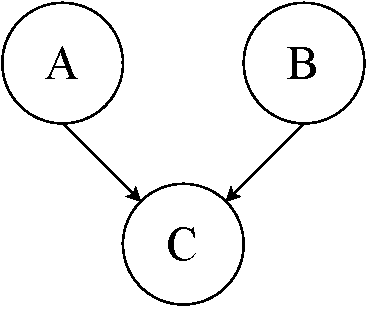
\includegraphics[width=0.35\linewidth]{img/_cpt_graph.pdf}
                    \end{minipage}
                    \begin{minipage}{.48\linewidth}
                        \centering
                        \begin{tabular}{c|c|c|c}
                            A           & B         & $\prob{c \vert A, B}$ & $\prob{\lnot c \vert A, B}$ \\
                            \hline
                            a           & b         & $\alpha$ & $1-\alpha$ \\
                            $\lnot$a    & b         & $\beta$ & $1-\beta$ \\
                            a           & $\lnot$b  & $\gamma$ & $1-\gamma$ \\
                            $\lnot$a    & $\lnot$b  & $\delta$ & $1-\delta$ \\
                        \end{tabular}
                    \end{minipage}
                \end{example}
        \end{description}

    \item[Reasoning patterns] \marginnote{Reasoning patterns}
        Given a Bayesian network, the following reasoning patterns can be used:
        \begin{descriptionlist}
            \item[Causal] \marginnote{Causal reasoning}
                To make a prediction. From the cause, derive the effect.
                \begin{example}
                    Knowing $\texttt{Intelligence}$, it is possible to make a prediction of $\texttt{Letter}$.
                    \begin{center}
                        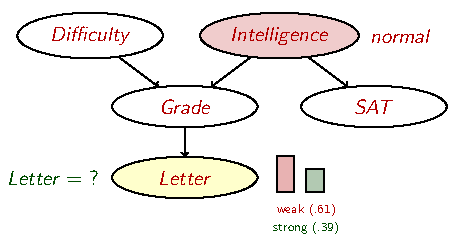
\includegraphics[width=0.5\linewidth]{img/_causal_example.pdf}
                    \end{center}
                \end{example}

            \item[Evidential] \marginnote{Evidential reasoning}
                To find an explanation. From the effect, derive the cause.
                \begin{example}
                    Knowing $\texttt{Grade}$, it is possible to explain it by estimating\\$\texttt{Intelligence}$.
                    \begin{center}
                        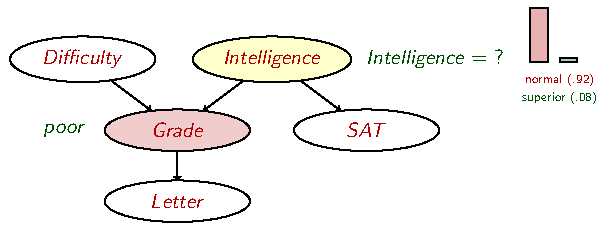
\includegraphics[width=0.7\linewidth]{img/_evidential_example.pdf}
                    \end{center}
                \end{example}

            \item[Explain away] \marginnote{Explain away reasoning}
                Observation obtained "passing through" other observations.
                \begin{example}
                    Knowing $\texttt{Difficulty}$ and $\texttt{Grade}$, 
                    it is possible to estimate \\$\texttt{Intelligence}$.

                    Note that if $\texttt{Grade}$ was not known, 
                    $\texttt{Difficulty}$ and $\texttt{Intelligence}$ would have been independent.
                    \begin{center}
                        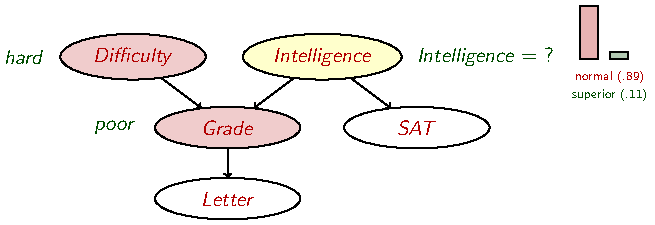
\includegraphics[width=0.75\linewidth]{img/_explainaway_example.pdf}
                    \end{center}
                \end{example}
        \end{descriptionlist}

    \item[Independence] \marginnote{Bayesian network independence}
        Intuitively, an effect is independent from a cause, 
        if there is another cause in the middle whose value is already known.
        \begin{example}
            \phantom{}

            \begin{minipage}{.3\linewidth}
                \centering
                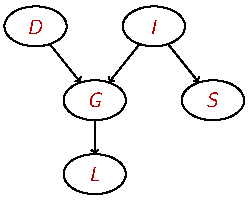
\includegraphics[width=0.85\linewidth]{img/_independence_example.pdf}
            \end{minipage}
            \begin{minipage}{.6\linewidth}
                \[ \textbf{P} \models (\texttt{L} \perp \texttt{D}, \texttt{I}, \texttt{S} \,\vert\, \texttt{G}) \]
                \[ \textbf{P} \models (\texttt{S} \perp \texttt{L} \,\vert\, \texttt{G}) \]
                \[ \textbf{P} \models (\texttt{S} \perp \texttt{D}) \text{ but } 
                    \textbf{P} \models (\texttt{S} \,\cancel{\perp}\, \texttt{D} \,\vert\, \texttt{G}) \text{ (explain away)} \]
            \end{minipage}
        \end{example}


    \item[V-structure] \marginnote{V-structure}
        Effect with two causes.
        If the effect is not in the evidence, the causes are independent.

        \begin{figure}[H]
            \centering
            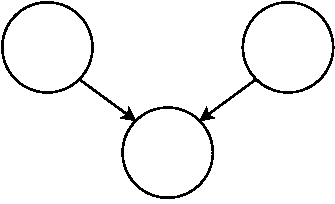
\includegraphics[width=0.2\textwidth]{img/_v_structure.pdf}
            \caption{V-structure}
        \end{figure}
    
    \item[Active two-edge trail] \marginnote{Active two-edge trail}
        The trail $X \leftrightharpoons Z \leftrightharpoons Y$ is active either if:
        \begin{itemize}
            \item $X$, $Z$, $Y$ is a v-structure $X \rightarrow Z \leftarrow Y$
                and $Z$ or one of its children is in the evidence.
            \item $Z$ is not in the evidence.
        \end{itemize}
        In other words, influence can flow from $X$ to $Y$ passing by $Z$.

        \begin{figure}[h]
            \centering
            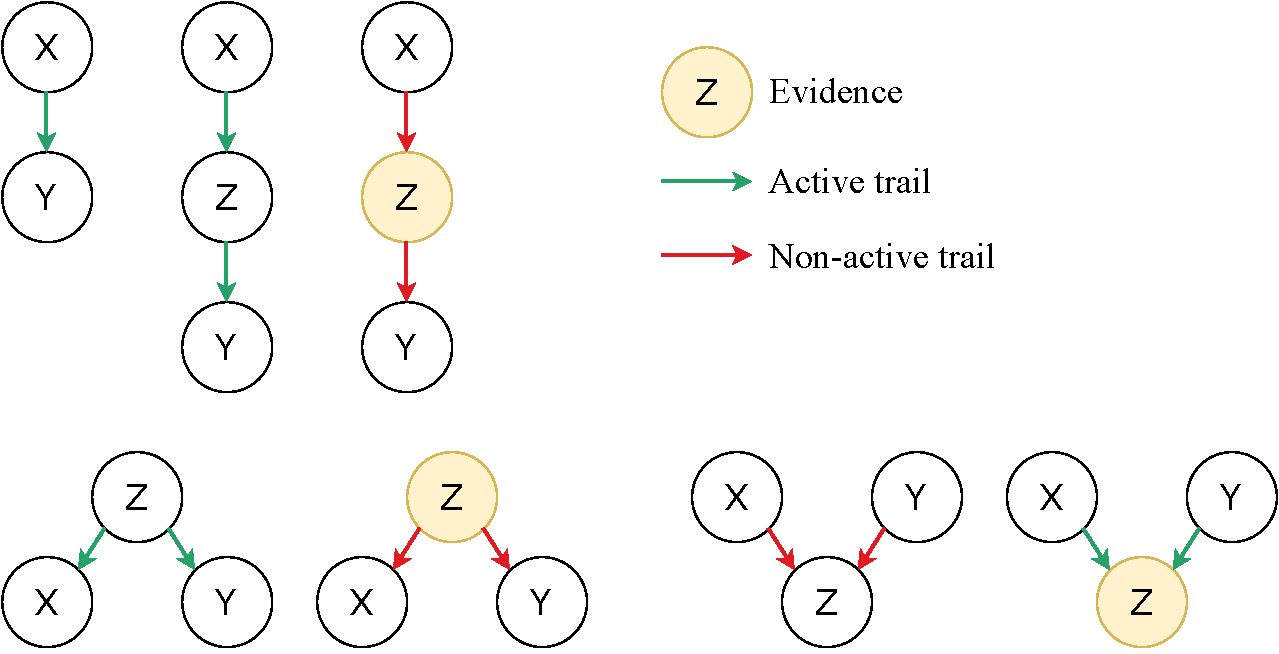
\includegraphics[width=0.65\textwidth]{img/_active_trail.pdf}
            \caption{Example of active and non-active two-edge trails}
        \end{figure}
    
    \item[Active trail] \marginnote{Active trail}
        A trail $X_1 \leftrightharpoons \dots \leftrightharpoons X_n$ is active iff
        each two-edge trail $X_{i-1} \leftrightharpoons X_i \leftrightharpoons X_{i+1}$ along the trail is active.

    \item[D-separation] \marginnote{D-separation}
        Two sets of nodes $\vec{X}$ and $\vec{Y}$ are d-separated given the evidence $\vec{Z}$ if
        there is no active trail between any $X \in \vec{X}$ and $Y \in \vec{Y}$.

        \begin{theorem}
            Two d-separated nodes are independent.
            In other words, two nodes are independent if there is no active trail between them.
        \end{theorem}

    \item[Independence algorithm] \phantom{}
        \begin{description}
            \item[Blocked node]
                A node is blocked if it blocks the flow.
                This happens if one and only one of the following conditions are met:
                \begin{itemize}
                    \item The node is in the middle of an unmarked v-structure.
                    \item The node is in the evidence.
                \end{itemize}
        \end{description}
        To determine if $X \perp Y$ given the evidence $\vec{Z}$:
        \begin{enumerate}
            \item Traverse the graph bottom-up marking all nodes in $\vec{Z}$ or
                having a child in $\vec{Z}$.
            \item Find a path from $X$ to $Y$ that does not pass through a blocked node.
            \item If $Y$ is not reachable from $X$, then $X$ and $Y$ are independent.
                Otherwise $X$ and $Y$ are dependent.
        \end{enumerate}

        \begin{example}
            To determine if $J \perp D$:
            \begin{center}
                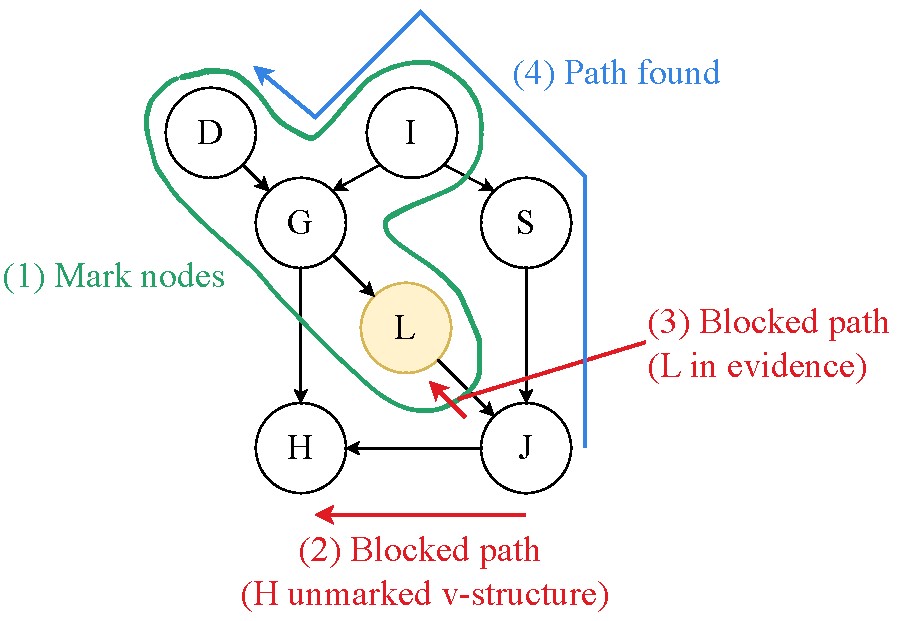
\includegraphics[width=0.5\textwidth]{img/_d_sep_example.pdf}
            \end{center}
            As a path has been found, $J \,\cancel{\perp}\, D$.
        \end{example}
    

    \item[Global semantics] \marginnote{Global semantics}
        Given a Bayesian network, the full joint distribution can be defined as
        the product of the local conditional distributions:
        \[ \prob{x_1, \dots, x_n} = \prod_{i=1}^{n} \prob{x_i \,\vert\, \texttt{parents}(X_i)} \]

        \begin{example}
            Given the following Bayesian network:

            \begin{minipage}{.3\linewidth}
                \centering
                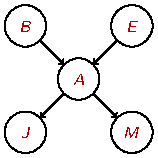
\includegraphics[width=0.7\linewidth]{img/_global_semantics_example.pdf}
            \end{minipage}
            \begin{minipage}{.6\linewidth}
                \[ 
                    \begin{split}
                        &\prob{j \land m \land a \land \lnot b \land \lnot e} \\
                            &= \prob{\lnot b} \prob{\lnot e} \prob{a \,\vert\, \lnot b, \lnot e}
                                \prob{j \,\vert\, a} \prob{m \,\vert\, a}
                    \end{split}
                \]
            \end{minipage}
        \end{example}

    \item[Local semantics]
        Each node is conditionally independent of its non-descendants given its parents.
        \begin{figure}[h]
            \centering
            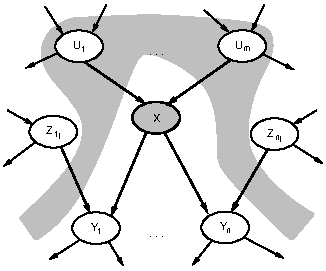
\includegraphics[width=0.35\textwidth]{img/_local_independence.pdf}
            \caption{Local independence}
        \end{figure}

        \begin{theorem}
            Local semantics $\iff$ Global semantics
        \end{theorem}
        
    
    \item[Markov blanket]
        Each node is conditionally independent of all other nodes 
        if its Markov blanket (parents, children, children's parents) is in the evidence.
        \begin{figure}[h]
            \centering
            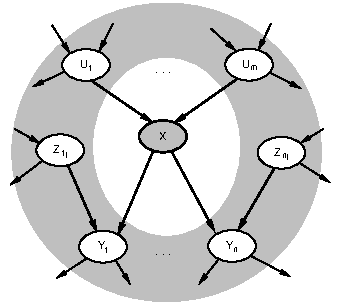
\includegraphics[width=0.35\textwidth]{img/_markov_blanket.pdf}
            \caption{Markov blanket}
        \end{figure}
\end{description}



\section{Building Bayesian networks}

\subsection{Algorithm}
The following algorithm can be used to construct a Bayesian network of $n$ random variables:
\begin{enumerate}
    \item Choose an ordering of the variables $X_1, \dots, X_n$.
    \item For $i=1, \dots, n$:
        \begin{itemize}
            \item Add $X_i$ to the network.
            \item Select the parents of $X_i$ from $X_1, \dots, X_{i-1}$ such that:
                \[ \textbf{P}(X_i \,\vert\, \texttt{parents}(X_i)) = 
                    \textbf{P}(X_i \,\vert\, X_1, \dots, X_{i-1}) \]
        \end{itemize}
\end{enumerate}
By construction, this algorithm guarantees the global semantics.

\begin{example}[Monty Hall]
    The variables are:
    \begin{itemize}
        \item $G$: the choice of the guest.
        \item $H$: the choice of the host.
        \item $P$: the position of the prize.
    \end{itemize}
    Note that $P \perp G$.
    Let the order be fixed as follows: $P$, $G$, $H$.

    \begin{figure}[h]
        \begin{subfigure}{.3\textwidth}
            \centering
            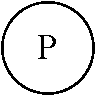
\includegraphics[width=0.15\linewidth]{img/_monty_hall1.pdf}
            \caption{First interaction}
        \end{subfigure}
        \begin{subfigure}{.3\textwidth}
            \centering
            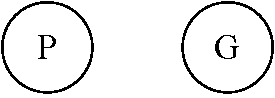
\includegraphics[width=0.45\linewidth]{img/_monty_hall2.pdf}
            \caption{Second interaction (note that $P \perp G$)}
        \end{subfigure}
        \begin{subfigure}{.3\textwidth}
            \centering
            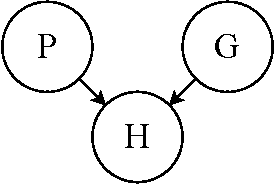
\includegraphics[width=0.45\linewidth]{img/_monty_hall3.pdf}
            \caption{Third interaction}
        \end{subfigure}
    \end{figure}
\end{example}

The nodes of the resulting network can be classified as:
\begin{descriptionlist}
    \item[Initial evidence] The initial observation.
    \item[Testable variables] Variables that can be verified.
    \item[Operable variables] Variables that can be changed by intervening on them.
    \item[Hidden variables] Variables that "compress" more variables to reduce the parameters.
\end{descriptionlist}

\begin{example} \phantom{}\\
    \begin{minipage}{.4\linewidth}
        \begin{description}
            \item[Initial evidence] Red.
            \item[Testable variables] Green.
            \item[Operable variables] Orange.
            \item[Hidden variables] Gray.
        \end{description}
    \end{minipage}
    \begin{minipage}{.5\linewidth}
        \begin{center}
            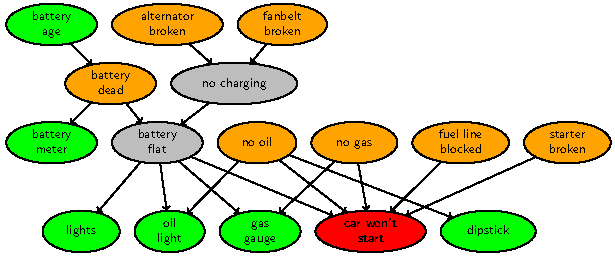
\includegraphics[width=\linewidth]{img/_car_example.pdf}
        \end{center}
    \end{minipage}
\end{example}


\subsection{Structure learning}
\marginnote{Structure learning}
Learn the network from the available data.
\begin{description}
    \item[Constraint-based] 
        Independence tests to identify the constraints of the edges.
    \item[Score-based] 
        Define a score to evaluate the network.
\end{description}



\section{Causal networks}
When building a Bayesian network, a correct ordering of the nodes 
that respects the causality allows to obtain more compact networks.

\begin{description}
    \item[Structural equation] \marginnote{Structural equation}
        Given a variable $X_i$ with values $x_i$, its structural equation is a function $f_i$
        such that it represents all its possible values:
        \[ x_i = f_i(\text{other variables}, U_i) \]
        $U_i$ represents unmodeled variables or error terms.

    \item[Causal network] \marginnote{Causal network}
        Restricted class of Bayesian networks that only allows causally compatible ordering.

        An edge exists between $X_j \rightarrow X_i$ iff $X_j$ is an argument of 
        the structural equation $f_i$ of $X_i$.

        \begin{example} \phantom{}\\[0.5em]
            \begin{minipage}{.3\linewidth}
                \centering
                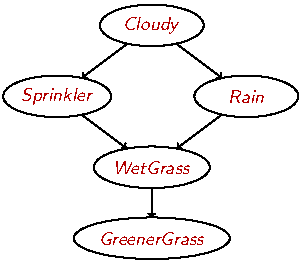
\includegraphics[width=\linewidth]{img/_causal_network_example1.pdf}
            \end{minipage}
            \begin{minipage}{.6\linewidth}
                The structural equations are:
                \[ 
                    \begin{split}
                        \texttt{cloudy} &= f_C(U_C) \\
                        \texttt{sprinkler} &= f_S(\texttt{Cloudy}, U_S) \\
                        \texttt{rain} &= f_R(\texttt{Cloudy}, U_R) \\
                        \texttt{wet\_grass} &= f_W(\texttt{Sprinkler}, \texttt{Rain}, U_W) \\
                        \texttt{greener\_grass} &= f_G(\texttt{WetGrass}, U_G)
                    \end{split}
                \]
            \end{minipage}\\[0.5em]

            If the sprinkler is disabled, the network becomes:\\[0.5em]
            \begin{minipage}{.3\linewidth}
                \centering
                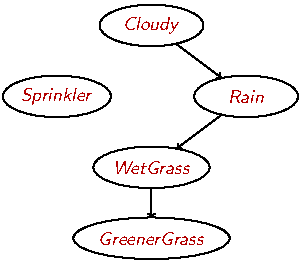
\includegraphics[width=\linewidth]{img/_causal_network_example2.pdf}
            \end{minipage}
            \begin{minipage}{.6\linewidth}
                The structural equations become:
                \[ 
                    \begin{split}
                        \texttt{cloudy} &= f_C(U_C) \\
                        \texttt{sprinkler} &= f_S(U_S) \\
                        \texttt{rain} &= f_R(\texttt{Cloudy}, U_R) \\
                        \texttt{wet\_grass} &= f_W(\texttt{Rain}, U_W) \\
                        \texttt{greener\_grass} &= f_G(\texttt{WetGrass}, U_G)
                    \end{split}
                \]
            \end{minipage}
        \end{example}

    \item[do-operator] \marginnote{do-operator}
        The do-operator allows to represent manual interventions on the network.
        The operation $\texttt{do}(X_i = x_i)$ makes the structural equation of $X_i$
        constant (i.e. $f_i = x_i$, without arguments, so there won't be inward edges to $X_i$).

        \begin{example} \phantom{}\\[0.5em]
            \begin{minipage}{.3\linewidth}
                \centering
                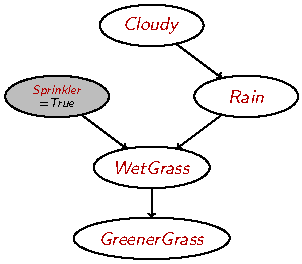
\includegraphics[width=\linewidth]{img/_do_operator_example1.pdf}
            \end{minipage}
            \begin{minipage}{.65\linewidth}
                By applying $\texttt{do}(\texttt{Sprinkler} = \texttt{true})$, the structural equations become:
                \[ 
                    \begin{split}
                        \texttt{cloudy} &= f_C(U_C) \\
                        \texttt{sprinkler} &= \texttt{true} \\
                        \texttt{rain} &= f_R(\texttt{Cloudy}, U_R) \\
                        \texttt{wet\_grass} &= f_W(\texttt{Sprinkler}, \texttt{Rain}, U_W) \\
                        \texttt{greener\_grass} &= f_G(\texttt{WetGrass}, U_G)
                    \end{split}
                \]
            \end{minipage}\\[0.5em]

            \begin{minipage}{.3\linewidth}
                \centering
                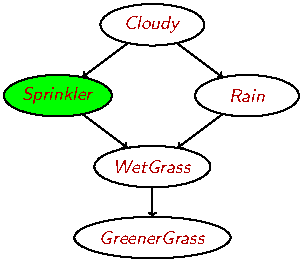
\includegraphics[width=\linewidth]{img/_do_operator_example2.pdf}
            \end{minipage}
            \begin{minipage}{.65\linewidth}
                Note that Bayesian networks are not capable of modelling manual interventions.
                In fact, intervening and observing a variable are different concepts:
                \[ \prob{\texttt{WetGrass} \mid \texttt{do}(\texttt{Sprinkler} = \texttt{true})} \]
                \[ \neq \]
                \[ \prob{\texttt{WetGrass} \mid \texttt{Sprinkler} = \texttt{true}} \]
            \end{minipage}
        \end{example}
\end{description}



\section{Compact conditional distributions}

Use canonical distributions (standard patterns) to reduce 
the number of variables in a conditional probability table.


\subsection{Noisy-OR}
\marginnote{Noisy-OR}
Noisy-OR distributions model a network of non-interacting causes with a common effect.
A node $X$ has $k$ parents $U_1, \dots, U_k$ and possibly a leak node $U_L$ to capture unmodeled concepts. 

\begin{figure}[h]
    \centering
    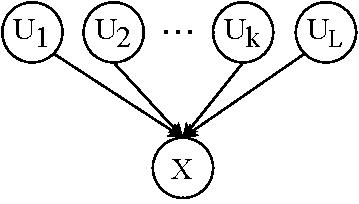
\includegraphics[width=0.3\textwidth]{img/_noisy_or_example.pdf}
    \caption{Example of noisy-OR network}
\end{figure}

Each node $U_i$ has a failure (inhibition) probability $q_i$:
\[ q_i = \prob{\lnot x \mid u_i, \lnot u_j \text{ for } j \neq i} \]
The CPT can be built by computing the probabilities as:
\[ \prob{\lnot x \mid \texttt{Parents($X$)}} = \prod_{j:\, U_j = \texttt{true}} q_j \]
In other words:
\[ \prob{\lnot x \mid u_1, \dots, u_n} = 
    \prob{\lnot x \mid u_1} \cdot \prob{\lnot x \mid u_2} \cdot \text{\dots} \cdot \prob{\lnot x \mid u_n} \]

Because only the failure probabilities are required, the number of parameters is linear in the number of parents.

\begin{example}
    We have as causes \texttt{Cold}, \texttt{Flu} and \texttt{Malaria} and as effect \texttt{Fever}.
    For simplicity there are no leak nodes.
    The failure probabilities are:
    \[
        \begin{split}
            q_\texttt{cold} &= \prob{\lnot \texttt{fever} \mid \texttt{cold}, \lnot\texttt{flu}, \lnot\texttt{malaria}} = 0.6 \\
            q_\texttt{flu} &= \prob{\lnot \texttt{fever} \mid \lnot\texttt{cold}, \texttt{flu}, \lnot\texttt{malaria}} = 0.2 \\
            q_\texttt{malaria} &= \prob{\lnot \texttt{fever} \mid \lnot\texttt{cold}, \lnot\texttt{flu}, \texttt{malaria}} = 0.1
        \end{split}    
    \]

    Known the failure probabilities, the entire CPT can be computed:
    \begin{center}
        \begin{tabular}{c|c|c|rc|c}
            \hline
            \texttt{Cold} & \texttt{Flu} & \texttt{Malaria} & \multicolumn{2}{c|}{$\prob{\lnot\texttt{fever}}$} & $1-\prob{\lnot\texttt{fever}}$ \\
            \hline
            F & F & F &                                                                 & 0.0       & 1.0 \\
            F & F & T & $q_\texttt{malaria} =$                                            & 0.1       & 0.9 \\
            F & T & F & $q_\texttt{flu} =$                                                & 0.2       & 0.8 \\
            F & T & T & $q_\texttt{flu} \cdot q_\texttt{malaria} =$                       & 0.02      & 0.98 \\
            T & F & F & $q_\texttt{cold} =$                                               & 0.6       & 0.4 \\
            T & F & T & $q_\texttt{cold} \cdot q_\texttt{malaria} =$                      & 0.06      & 0.94 \\
            T & T & F & $q_\texttt{cold} \cdot q_\texttt{flu} =$                          & 0.12      & 0.88 \\
            T & T & T & $q_\texttt{cold} \cdot q_\texttt{flu} \cdot q_\texttt{malaria} =$ & 0.012     & 0.988 \\
            \hline
        \end{tabular}
    \end{center}
\end{example}


\subsection{Hybrid Bayesian networks}
\marginnote{Hybrid Bayesian networks}

Network with discrete and continuous random variables.
Continuous variables must be converted into a finite representation.
Possible approaches are:
\begin{description}
    \item[Discretization] \marginnote{Discretization} 
        Values are divided into a fixed set of intervals.
        This approach may introduce large errors and large CPTs.

    \item[Finitely parametrized canonical families] \marginnote{Finitely parametrized canonical families}
        There are two cases to handle using this approach:
        \begin{descriptionlist}
            \item[Continuous child] 
                Given the continuous variables $X$ and $C$ and a discrete (boolean, for simplicity) variable $D$,
                we want to compute the distribution $\textbf{P}(X \mid C, D)$.

                The discrete parent is handled by enumeration, by computing the probability over the domain of $D$.

                For the continuous parent, an arbitrarily chosen distribution over the values of $X$ is used.
                A common choice is the \textbf{linear Gaussian} \marginnote{Linear Gaussian}
                whose mean is a linear combination of the values of the parents and the variance is fixed.
                
                A network with all continuous linear Gaussian distributions has the property 
                of having a multivariate Gaussian distribution as joint distribution.
                Moreover, if a continuous variable has some discrete parents, it defines a conditional Gaussian distribution
                where, fixed the values of the discrete variables, the distribution over the continuous variable is a multivariate Gaussian.

                \begin{example}
                    Let \texttt{Subsidy} and \texttt{Buys} be discrete variables and
                    \texttt{Harvest} and \texttt{Cost} be continuous variables.
                    \begin{center}
                        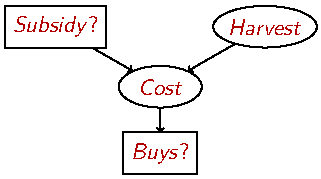
\includegraphics[width=0.3\textwidth]{img/_linear_gaussian_example.pdf}
                    \end{center}
    
                    To compute $\textbf{P}(\texttt{Cost} \mid \texttt{Harvest}, \texttt{Subsidy})$,
                    we split the probabilities over the values of the discrete variable \texttt{Subsidy}
                    and use a linear Gaussian for \texttt{Harvest}.
                    We therefore have that:
                    \[ 
                        \begin{split}
                            \prob{\texttt{C} = \texttt{c} \mid \texttt{Harvest} = \texttt{h}, \texttt{Subsidy} = \texttt{true}} 
                            &= \mathcal{N}(a_t h + b_t, \sigma_t)(c) \\
                            \prob{\texttt{C} = \texttt{c} \mid \texttt{Harvest} = \texttt{h}, \texttt{Subsidy} = \texttt{false}} 
                            &= \mathcal{N}(a_f h + b_f, \sigma_f)(c)
                        \end{split}
                    \]
                    where $a_t$, $b_t$, $\sigma_t$, $a_f$, $b_f$ and $\sigma_t$ are parameters.
                \end{example}

            \item[Discrete child with continuous parents] 
                Given the continuous variable $C$ and a discrete variable $X$,
                the probability of $X$ given $C$ in obtained by using a threshold function.
                For instance, probit or sigmoid distributions can be used.
        \end{descriptionlist}
\end{description}


\subsection{Other methods}

\begin{description}
    \item[Dynamic Bayesian network] \marginnote{Dynamic Bayesian network}
        Useful to model the evolution through time.
        A template variable $X_i$ is instantiated as $X_i^{(t)}$ at each time step.
        \begin{figure}[h]
            \centering
            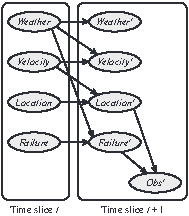
\includegraphics[width=0.3\textwidth]{img/_dynamic_bn_example.pdf}
            \caption{Example of dynamic Bayesian network}
        \end{figure}

    \item[Density estimation] \marginnote{Density estimation}
        Parameters of the conditional distribution can be learned using:
        \begin{description}
            \item[Bayesian learning] calculate the probability of each hypothesis.
            \item[Approximations] using the maximum-a-posteriori and maximum-likelihood hypothesis.
            \item[Expectation-maximization algorithm{\normalfont.}] 
        \end{description}

    \item[Undirected graphical models] \marginnote{Undirected graphical models}
        Markov networks are an alternative to probabilistic graphical models (as Bayesian networks).
        Markov networks are undirected graphs with factors (instead of probabilities) and
        are able to naturally capture independence relations.
\end{description}